% =============================================================================
% practica8.tex --- Chapter: Practice 8
% =============================================================================

\documentclass[../../__memoria.tex]{subfiles}

\begin{document}
\standalonecover
\pagestyle{cuerpo}

\graphicspath{{\subfix{../../Imagenes/}}{../../Imagenes/}{\subfix{img/}}{img/}}

\chapter[Práctica 8: Aprendizaje Activo]{Cuaderno de Laboratorio --- Práctica 8: Aprendizaje Activo}

\section*{Introducción}
En esta práctica trabajamos con \textit{Active Learning} (Aprendizaje Activo), una técnica especialmente útil cuando etiquetar datos es caro o lento. La idea es que el modelo no reciba datos etiquetados de forma pasiva, sino que sea él mismo quien elija qué muestras merecen la pena etiquetar. Para comparar si esto realmente funciona, enfrentamos dos estrategias: seleccionar puntos al azar (línea base) y seleccionar los puntos donde el modelo tiene más dudas (aprendizaje activo por incertidumbre).

Usamos el dataset sintético \textit{make\_moons}, que genera dos clases en forma de medias lunas. Empezamos con solo 10 puntos etiquetados y añadimos 5 en cada iteración hasta llegar a 50.

% -----------------------------------------------------------------------------
\section[Tarea 1: Entrenamiento Inicial]{Tarea 1 --- Entrenamiento Inicial con 10 Etiquetas}
% -----------------------------------------------------------------------------

El primer paso fue entrenar un \texttt{RandomForestClassifier} con los 10 puntos etiquetados iniciales y medir su rendimiento en el conjunto de test.

\textbf{Resultado:}
\begin{itemize}
    \item \textit{Accuracy} en test con 10 etiquetas: \textbf{0.7567}
\end{itemize}

Un 75.7\% con 10 puntos es un resultado razonablemente decente para tan poco dato, pero tiene problemas evidentes. Con tan pocas muestras, el modelo apenas ha visto el espacio de características: hay zonas enteras del dataset de las que no sabe nada. Además, los 10 puntos iniciales pueden no ser representativos por puro azar, lo que hace que el modelo sea bastante poco fiable. Cualquier evaluación con tan pocas muestras de entrenamiento tiene una varianza enorme: si los 10 puntos hubieran caído en otra zona del espacio, el accuracy podría ser muy distinto.

% -----------------------------------------------------------------------------
\section[Tarea 2: Baseline Aleatorio]{Tarea 2 --- Baseline: Selección Aleatoria}
% -----------------------------------------------------------------------------

Para tener una referencia con la que comparar el aprendizaje activo, implementamos primero una estrategia sin ninguna inteligencia: en cada iteración se seleccionan 5 puntos completamente al azar del pool no etiquetado, se consulta el oráculo para obtener sus etiquetas, y se añaden al conjunto de entrenamiento.

\textbf{Resultados de la selección aleatoria:}

\begin{center}
\begin{tabular}{cc}
\toprule
\textbf{Etiquetas usadas} & \textbf{Accuracy en test} \\
\midrule
10  & 0.7567 \\
15  & 0.8433 \\
20  & 0.8400 \\
25  & 0.8567 \\
30  & 0.8567 \\
35  & 0.9033 \\
40  & 0.9067 \\
45  & 0.9167 \\
50  & 0.9233 \\
\bottomrule
\end{tabular}
\end{center}

La selección aleatoria es la línea base porque representa lo que haríamos si no tuviéramos ninguna estrategia: etiquetar datos sin criterio. Sirve para medir cuánto aporta realmente el aprendizaje activo. Si la selección inteligente no supera a la aleatoria, significa que no está funcionando.

En este caso se ve que la curva sube de forma bastante irregular: hay saltos grandes (de 10 a 15 etiquetas sube 8 puntos), pero también momentos donde añadir más datos casi no mejora nada (de 20 a 25 la mejora es mínima). Esto es normal con selección aleatoria: a veces tocas puntos informativos, a veces no.

% -----------------------------------------------------------------------------
\section[Tarea 3: Active Learning por Incertidumbre]{Tarea 3 --- Selección por Incertidumbre}
% -----------------------------------------------------------------------------

La estrategia de aprendizaje activo que implementamos se basa en la incertidumbre del modelo: en cada iteración seleccionamos los 5 puntos del pool donde la probabilidad predicha para la clase~1 está más cerca de 0.5. Cuanto más cerca de 0.5, más confundido está el modelo sobre ese punto.

Técnicamente, calculamos $|p - 0.5|$ para cada muestra del pool (donde $p$ es la probabilidad de clase~1 según \texttt{predict\_proba}) y seleccionamos los 5 con el valor más bajo, es decir, los que generan más incertidumbre.

\textbf{Resultados de la selección por incertidumbre:}

\begin{center}
\begin{tabular}{cc}
\toprule
\textbf{Etiquetas usadas} & \textbf{Accuracy en test} \\
\midrule
10  & 0.7567 \\
15  & 0.8400 \\
20  & 0.8500 \\
25  & 0.9233 \\
30  & 0.9267 \\
35  & 0.9200 \\
40  & 0.9300 \\
45  & 0.9533 \\
50  & 0.9533 \\
\bottomrule
\end{tabular}
\end{center}

La diferencia más llamativa es que con solo 25 etiquetas la selección por incertidumbre ya alcanza el 92.3\%, un nivel que la selección aleatoria no consigue hasta las 50. Dicho de otra forma, el aprendizaje activo necesita la mitad de etiquetas para llegar al mismo rendimiento.

¿Por qué funcionan bien los puntos cercanos a la frontera? Porque son los puntos que más información aportan sobre dónde está el límite entre las dos clases. Un punto muy dentro de una región que el modelo ya clasificaba bien no cambia gran cosa la frontera de decisión; en cambio, un punto justo en la zona de duda le dice al modelo exactamente dónde trazar la línea divisoria. En \textit{make\_moons}, la frontera es curva y complicada, así que etiquetar los puntos que caen justo en esa zona es especialmente valioso.

% -----------------------------------------------------------------------------
\section[Tarea 4: Curva de Aprendizaje]{Tarea 4 --- Curva de Aprendizaje Comparativa}
% -----------------------------------------------------------------------------

\begin{center}
  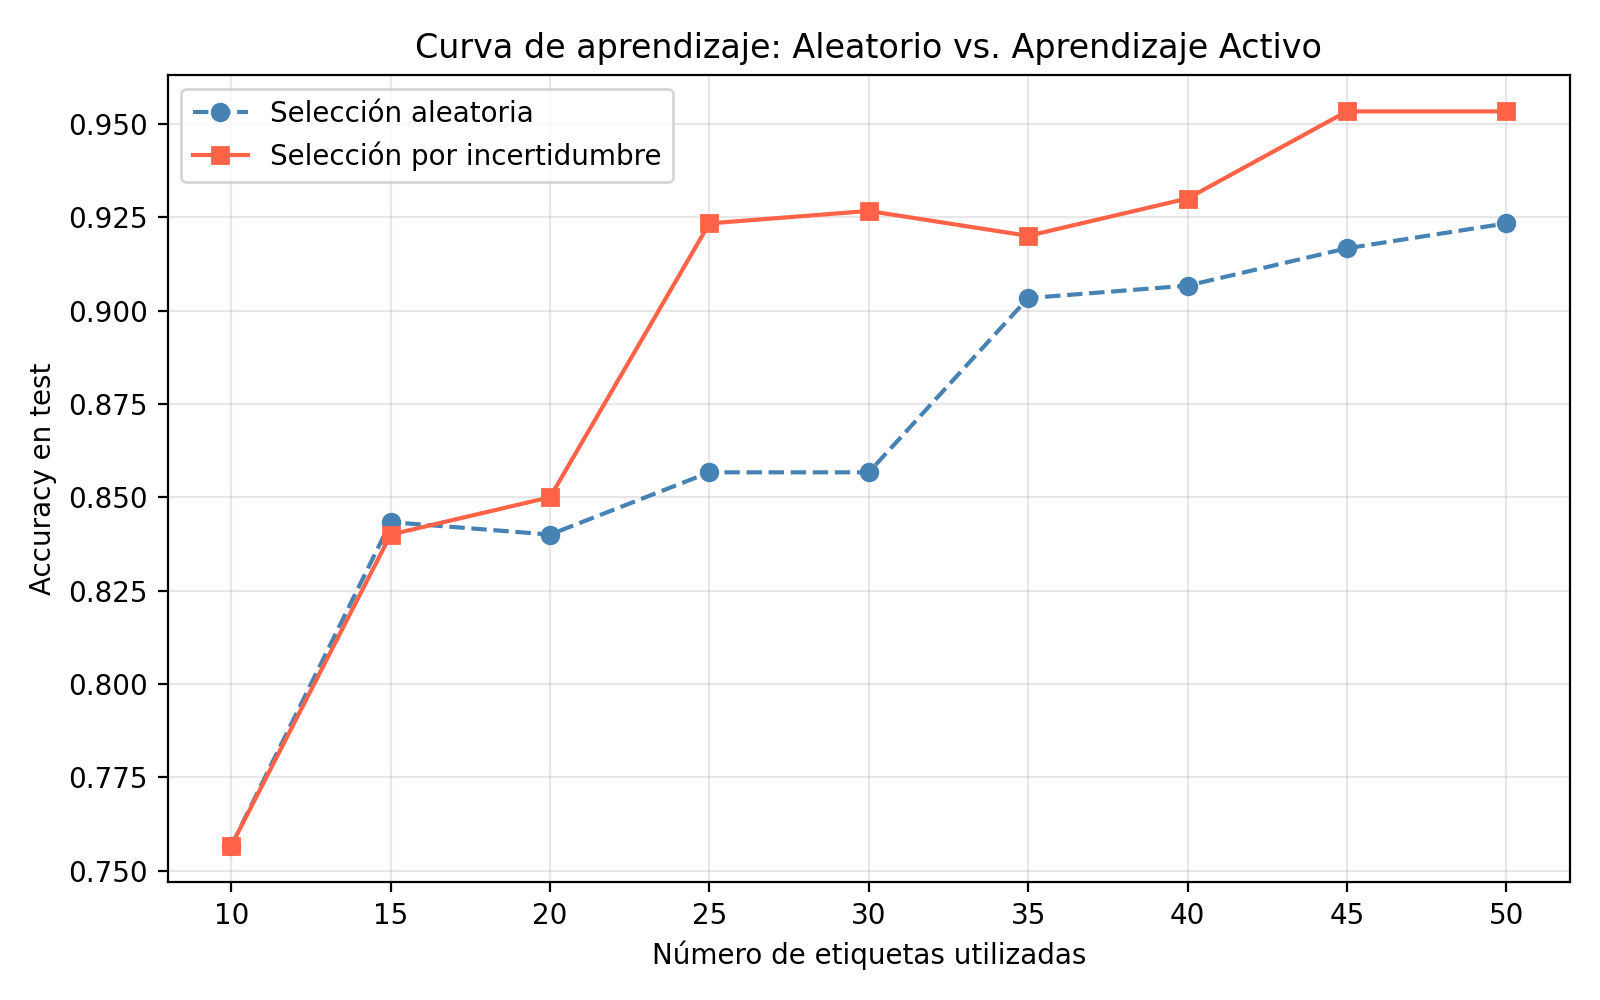
\includegraphics[width=0.88\linewidth]{img/learning_curve.png}
\end{center}

La gráfica muestra claramente la ventaja del aprendizaje activo. Ambas estrategias arrancan del mismo punto (0.7567 con 10 etiquetas, el mismo modelo inicial), pero a partir de 25 etiquetas la selección por incertidumbre se despega y se mantiene consistentemente por encima.

Al final, con 50 etiquetas:
\begin{itemize}
    \item Selección aleatoria: \textbf{0.9233}
    \item Selección por incertidumbre: \textbf{0.9533}
\end{itemize}

La curva de incertidumbre también es más estable: sube de forma más continua, sin los altibajos de la aleatoria. Esto tiene sentido porque la selección es dirigida; cada lote de puntos que se añade es útil por construcción.

% -----------------------------------------------------------------------------
\section[Tarea 5: Análisis Crítico]{Tarea 5 --- Análisis Crítico}
% -----------------------------------------------------------------------------

\textbf{¿Por qué el aprendizaje es más rápido cerca de la frontera?} \\
El modelo aprende la forma de la frontera de decisión. Los puntos que ya caen profundo en una zona bien clasificada no cambian esa frontera; el modelo ya sabe qué hacer con ellos. Pero los puntos que caen justo donde el modelo duda son exactamente la información que le falta: saber de qué lado de la línea están esos casos ambiguos le permite ajustar la frontera de manera mucho más precisa. Cada uno de esos puntos informativos equivale a varios puntos aleatorios en términos de mejora.

\vspace{0.3cm}

\textbf{¿Qué pasa si el modelo inicial es malo?} \\
Aquí está el talón de Aquiles del aprendizaje activo por incertidumbre. Si el modelo inicial es muy malo, sus probabilidades son poco fiables y la zona de ``incertidumbre'' que identifica puede no coincidir con la frontera real. En ese caso, los primeros lotes de puntos seleccionados pueden ser basura y el modelo no mejora, o incluso puede entrar en un ciclo donde siempre selecciona puntos de la misma zona sin explorar el resto. Este problema se conoce como \textit{exploitation vs.\ exploration}: el modelo explota su conocimiento actual (aunque sea erróneo) en lugar de explorar otras zonas.

Una forma de mitigarlo es combinar ambas estrategias: al principio, cuando el modelo es débil, seleccionar puntos más aleatoriamente para cubrir el espacio, y a medida que gana confianza, cambiar a selección por incertidumbre.

\vspace{0.3cm}

\textbf{¿Qué estrategia usaría en un caso real donde etiquetar cuesta dinero?} \\
En un caso real, creo que empezaría con selección aleatoria hasta tener un modelo mínimamente decente, y luego pasaría a incertidumbre. Esta práctica muestra que la selección por incertidumbre alcanza el mismo rendimiento con la mitad de etiquetas, pero eso asume que el modelo inicial es razonable. Si empiezo con un modelo muy malo, sus estimaciones de incertidumbre pueden no ser fiables, por lo que una fase inicial aleatoria ayuda a explorar el espacio antes de explotar.

% -----------------------------------------------------------------------------
\section*{Conclusión}

Lo que más me ha gustado de esta práctica es ver cómo el modelo puede decidir por sí mismo qué datos le conviene aprender. La diferencia entre seleccionar puntos al azar y seleccionar los que generan más dudas es muy clara: con la mitad de etiquetas se consigue el mismo rendimiento. Al principio me costó entender por qué \texttt{np.argsort()} ascendente servía para seleccionar los más inciertos (porque ordena de menor a mayor $|p-0.5|$), pero una vez visto es muy sencillo.

Si tuviese que aplicar aprendizaje activo en un problema real, creo que combinaría ambas estrategias: empezar con selección aleatoria para explorar y, cuando el modelo tenga cierta base, pasar a incertidumbre para afinar. Pero está claro que saber qué puntos etiquetar es casi tan importante como saber construir el modelo.

\vspace{3.0cm}

\end{document}
